Das Thema "`Daten und Informationen"' wird heutzutage immer wichtiger. Aber was beinhaltet Daten und Informationen alles? In der Steinzeit gab es die erste Form von Datenspeicherung in der Form von Höhlenmalereien. Bereits diese Bilder konnten "`Erfahrungen  mit Jagdwild, Jagdtechniken oder Wanderrouten von Tieren festhalten"' \cite{Hoehlenmalerei}. Wenn man dann weiter in die Zukunft schaut, erkennt man etwas revolutionäres in der Ägyptischen Kultur. Jedem Ägyptischen Zeichen wurde eine Bedeutung gegeben. Somit hatte man nun eine (teilweise) willkürliche Zuordnung von einem Zeichen für ein Objekt. Man musste also nun nicht mehr mit Bildern Informationen weitergeben, welche dann auch sehr verschieden interpretiert werden konnten, sondern man hatte eine Schrift entwickelt, die viel weniger Iterpretationsspielraum bot und dadurch auch viel präziser war. Genau diese Schrift hat uns dann, wenn auch mit einigen Modifikationen und Abstraktionen bis in die Neuzeit als effizienteste Datenspeicherung gedient. Natürlich gab es auch in dieser Zeit noch revolutionäre Erfindungen wie die Druckerpresse von Johannes Gutenberg. Aber der erste Schritt zur heutigen Datenspeicherung wurde erst vor 75 Jahren gemacht, als im Mai der "`Zuse Z3"'(Abbildung \ref{fig:Zuse_Z3}) fertiggestellt wurde, den man heute als den "`ersten funktionstüchtigen Computer der Geschichte"' bezeichnet. \cite{Computer} 
\begin{figure}[htbp] 
  \centering
     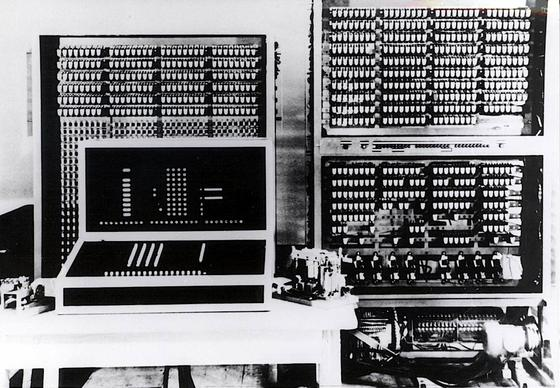
\includegraphics[width=0.7\textwidth]{Zuse_Z3.jpg}
  \caption{Zuse Z3 \cite{Zuse_Z3}}
  \label{fig:Zuse_Z3}
\end{figure}
Jedoch konnte dieser erste Computer, wie der Name bereits verrät (von eng. to compute = rechnen), die Daten nicht hauptsächlich speichern sondern verarbeiten. Und genau diese Datenverarbeitung ist es, die uns in den letzten Jahren so stark geprägt hat. Viele einfache Dinge, für die früher ein Mensch praktizieren musste, wird heute von einem Computer übernommen, der das ganze dann meistens auch noch viel schneller kann. Und genau diese Datenverarbeitung in Verbindung mit der Benutzerinteraktion steht bei unser Projektarbeit im Mittelpunkt. Das Ziel unseres Projekt ist es, dem Benutzer etwas beizubringen und das auf einem möglichst ertragreichem Weg. Das beizubringede wird auf Karten des Spiels "`Magic: The Gathering"'(Abbildung \ref{fig:Magiccard}) beschränkt.
\begin{figure}[htbp] 
  \centering
     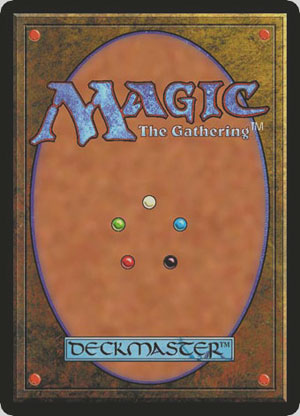
\includegraphics[width=0.4\textwidth]{Magiccard.jpg}
  \caption{Magickarte \cite{Magiccard}}
  \label{fig:Magiccard}
\end{figure}
Neben der Funktion mussten wir uns auch noch für eine Platform entscheiden, auf welcher unsere App verfügbar sein sollte. Da man jeder Zeit die Karten lernen können sollte, haben wir uns für eine mobile Android-App entschieden. Der Benutzer kann über ein Menu entscheiden, welche Karten er lernen will. Dann kann er über eine Lernfunktion die Karten lernen. Wie oben schon angeprochen, steht die Datenverarbeitung im Mittelpunkt. Deshalb speichern wir ab, ob der Benutzer die Karte gekonnt hat oder nicht. Falls ja, sollte die Karte in nächster Zukunft nicht noch einmal erscheinen, falls nein, sollte sie in naher Zukunft wieder erscheinen. Insofern kann man den maximalen Lernerfolg erreichen, da gezielt die Karten abgefragt werden, die noch nicht richtig sitzen. Ausserdem werden Daten auf zwei verschiedene Arten gespeichert: Einmal auf der App selbst und dann sollten diese auch noch ins Gedächniss des Benutzers gelangen. Natürlich sollte die App nicht nur funktionieren sondern auch noch ansprechend Aussehen und Benutzerfreundlich sein. Aber genau das ist es, was unsere App ausmachen soll: "`Magic2Brain"'